\section{Introduction}

%This template was produced using the \LaTeX type-setting system. It is
%more powerful than a WISIWIG word processor system such as Microsoft
%Word, especially when it comes to type-setting for code listings.
%See the text in the {\texttt{*.tex}} files for how to do this. A text editor such as
%Atom is suitable for writing the {\texttt{*.tex}} file. For more
%information on using \LaTeX~see~\cite{latex1} - an electronic resource
%from the library or see~\cite{latex2} for an online guide. You are
%free to use a word processor if you wish. Use this guide as a template
%for your report.
The aim of the project is to assess your ability to analyze, design
and implement an extension to an existing C/C++ program. The given program is a platform game that uses the SLD2 library for the graphics.

Your task is to extend the platform game starting from the provided skeleton code.
Hence, you must design at least one new feature, then adapt, modify and develop the code to realize this feature.
You are free to add any features you wish. You are required to write a
report describing the design and implementation of the changes you
make. You may develop it under Windows or Linux on the machines in the CS labs or on your own machine.

The assessment will take the form of a report on the game you develop.
You will be assessed on the complexity of your contribution and the quality of the report to document this contribution.The code will not be directly assessed although you must include a diff from your gitlab repository from the initial repository to the finished version.

\subsection{Learning Objectives}
\begin{itemize}
  \item Designing and implementing larger program in C/C++
  \item Managing the project development
  \item Report writing
\end{itemize}

\subsection{Provided Code}

You have been provided with a skeleton of a platform game which you
imported into the Visual Studio IDE in the tutorial for Week 1.
This skeleton uses the SLD2 library for graphics, sound, and keyboard interaction.
In Week 5, the tutorial was to follow the online tutorial from {\texttt{parallelrealities.co.uk}} on how the program had been constructed.

The skeleton code is written in C using {\em structs} as the main
data structure. You are free to develop the code in this style or to enrich it using C++ classes using an object orientation style.
Either way, you must justify you choice in the report and demonstrate this was
a sensible choice for the features you have employed.

\subsection{Suggested Approach}

You should use the practical session in G56 on Mondays, the drop-in
session on Mondays (G45), the CS1PR Slack channel and the programming
angel scheme to access help and support.
You may also help and receive
help from fellow students.
However, you should bare in mind this is an individual project make sure you submit only your own work.
See the University guidelines on plagiarism which are online.  

Your report should start with an {\textbf{Introduction}} section where
you introduce your work. What were the project goals, what features
did you wish to include in the game. Think about features of platform games you have played that
improve the game play. You may wish to include some of the following,
high scores, multiple levels, power-ups, enemies, movement parts
{\em etc}. 
You should justify what
programming style such as C/C++, did you use any OO features {\em etc}.

\section{Design}
Document what features you decided to implement and how they interact with
the rest of the game. Explain how the game play works.  
Include a diagram such as a flow
chart, \Cref{fig:fc} or UML diagram, \Cref{fig:uml}\footnote{Including
  both is allowed or even encouraged.}.

\begin{figure}[H]
\centering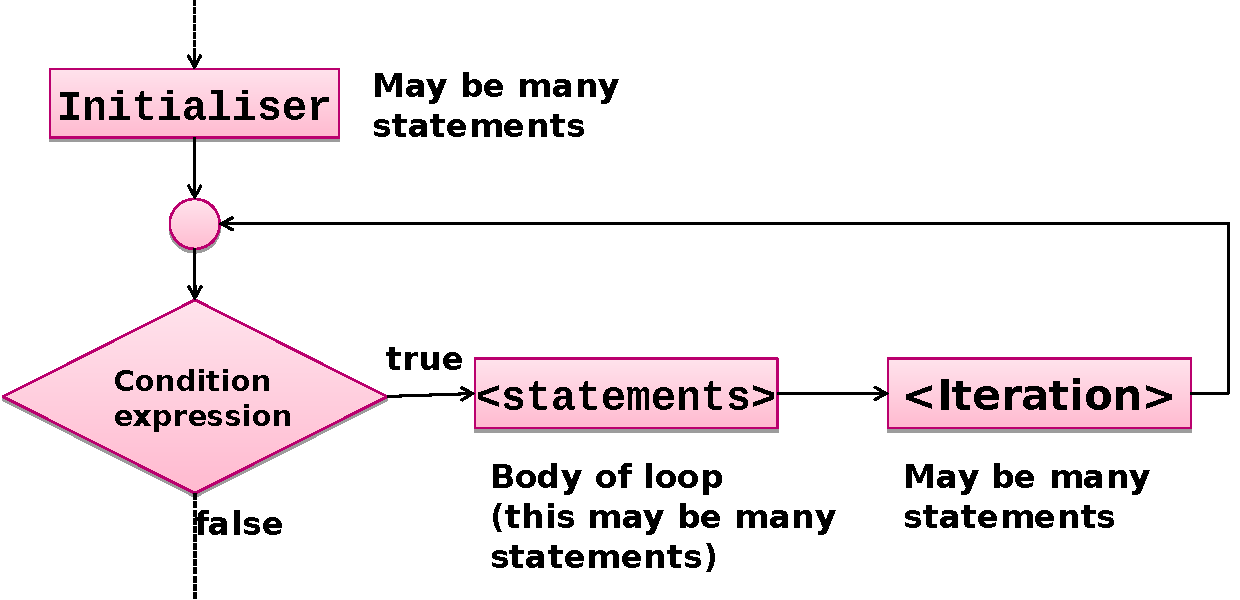
\includegraphics[width=0.66\linewidth]{simple-fc.pdf}
\caption{\label{fig:fc}A simple figure}
\end{figure}

\begin{figure}[H]
\centering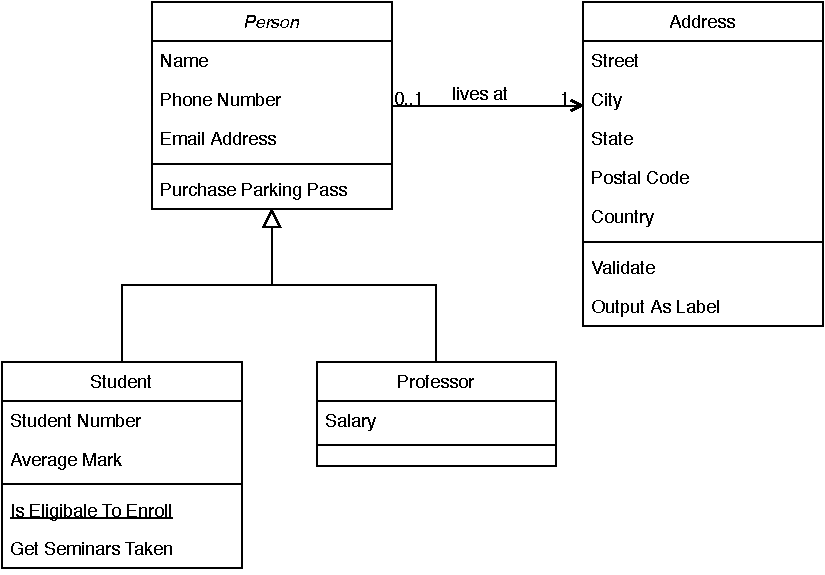
\includegraphics[width=0.75\linewidth]{simple-uml.pdf}
\caption{\label{fig:uml}A simple UML class diagram}
\end{figure}

In \Cref{lst:example}, you can see how to present a code example.
You can refer to specific sections of code using the line numbers, e.g., between Line~5-10, the setup is made, ...

\begin{lstfloat}
\lstinputlisting[label=lst:example,caption=My testcode (example.cpp) \attachfile{code/example.cpp}]{code/example.cpp}
\end{lstfloat}

\section{Implementation and Development}
Describe how you developed the code including what language features
you employed and why.
How did your program evolve from the original design?
Did you adapt the design to improve the game?
You should include code fragments and screen shots illustrate particular features.

Describe the finished game, including all the features you added.
What features work well?
Document any parts of the code which feel are important or
enable the program to work in a particular way.

Describe here your journey how you developed the program and reflect about your development.
How did you test and debug the program? Did you find all the bugs?
What testing have you employed to ensure the game works correctly. Did
you use any specific strategies for testing? 


\section{Conclusion}
Summarise your program development. What have your learnt about
programming? What have you learnt about developing a significant
program. What would either features would you add if you had more
time. What would you do differently?